\section{Resultados}\label{sec:resultados}
En la siguiente sección se presenta el entorno en que se trabaja y el gráfico que modela los resultados de la experiencia.

\subsection{Entorno de trabajo}

  \begin{figure}[H]
        \centering
        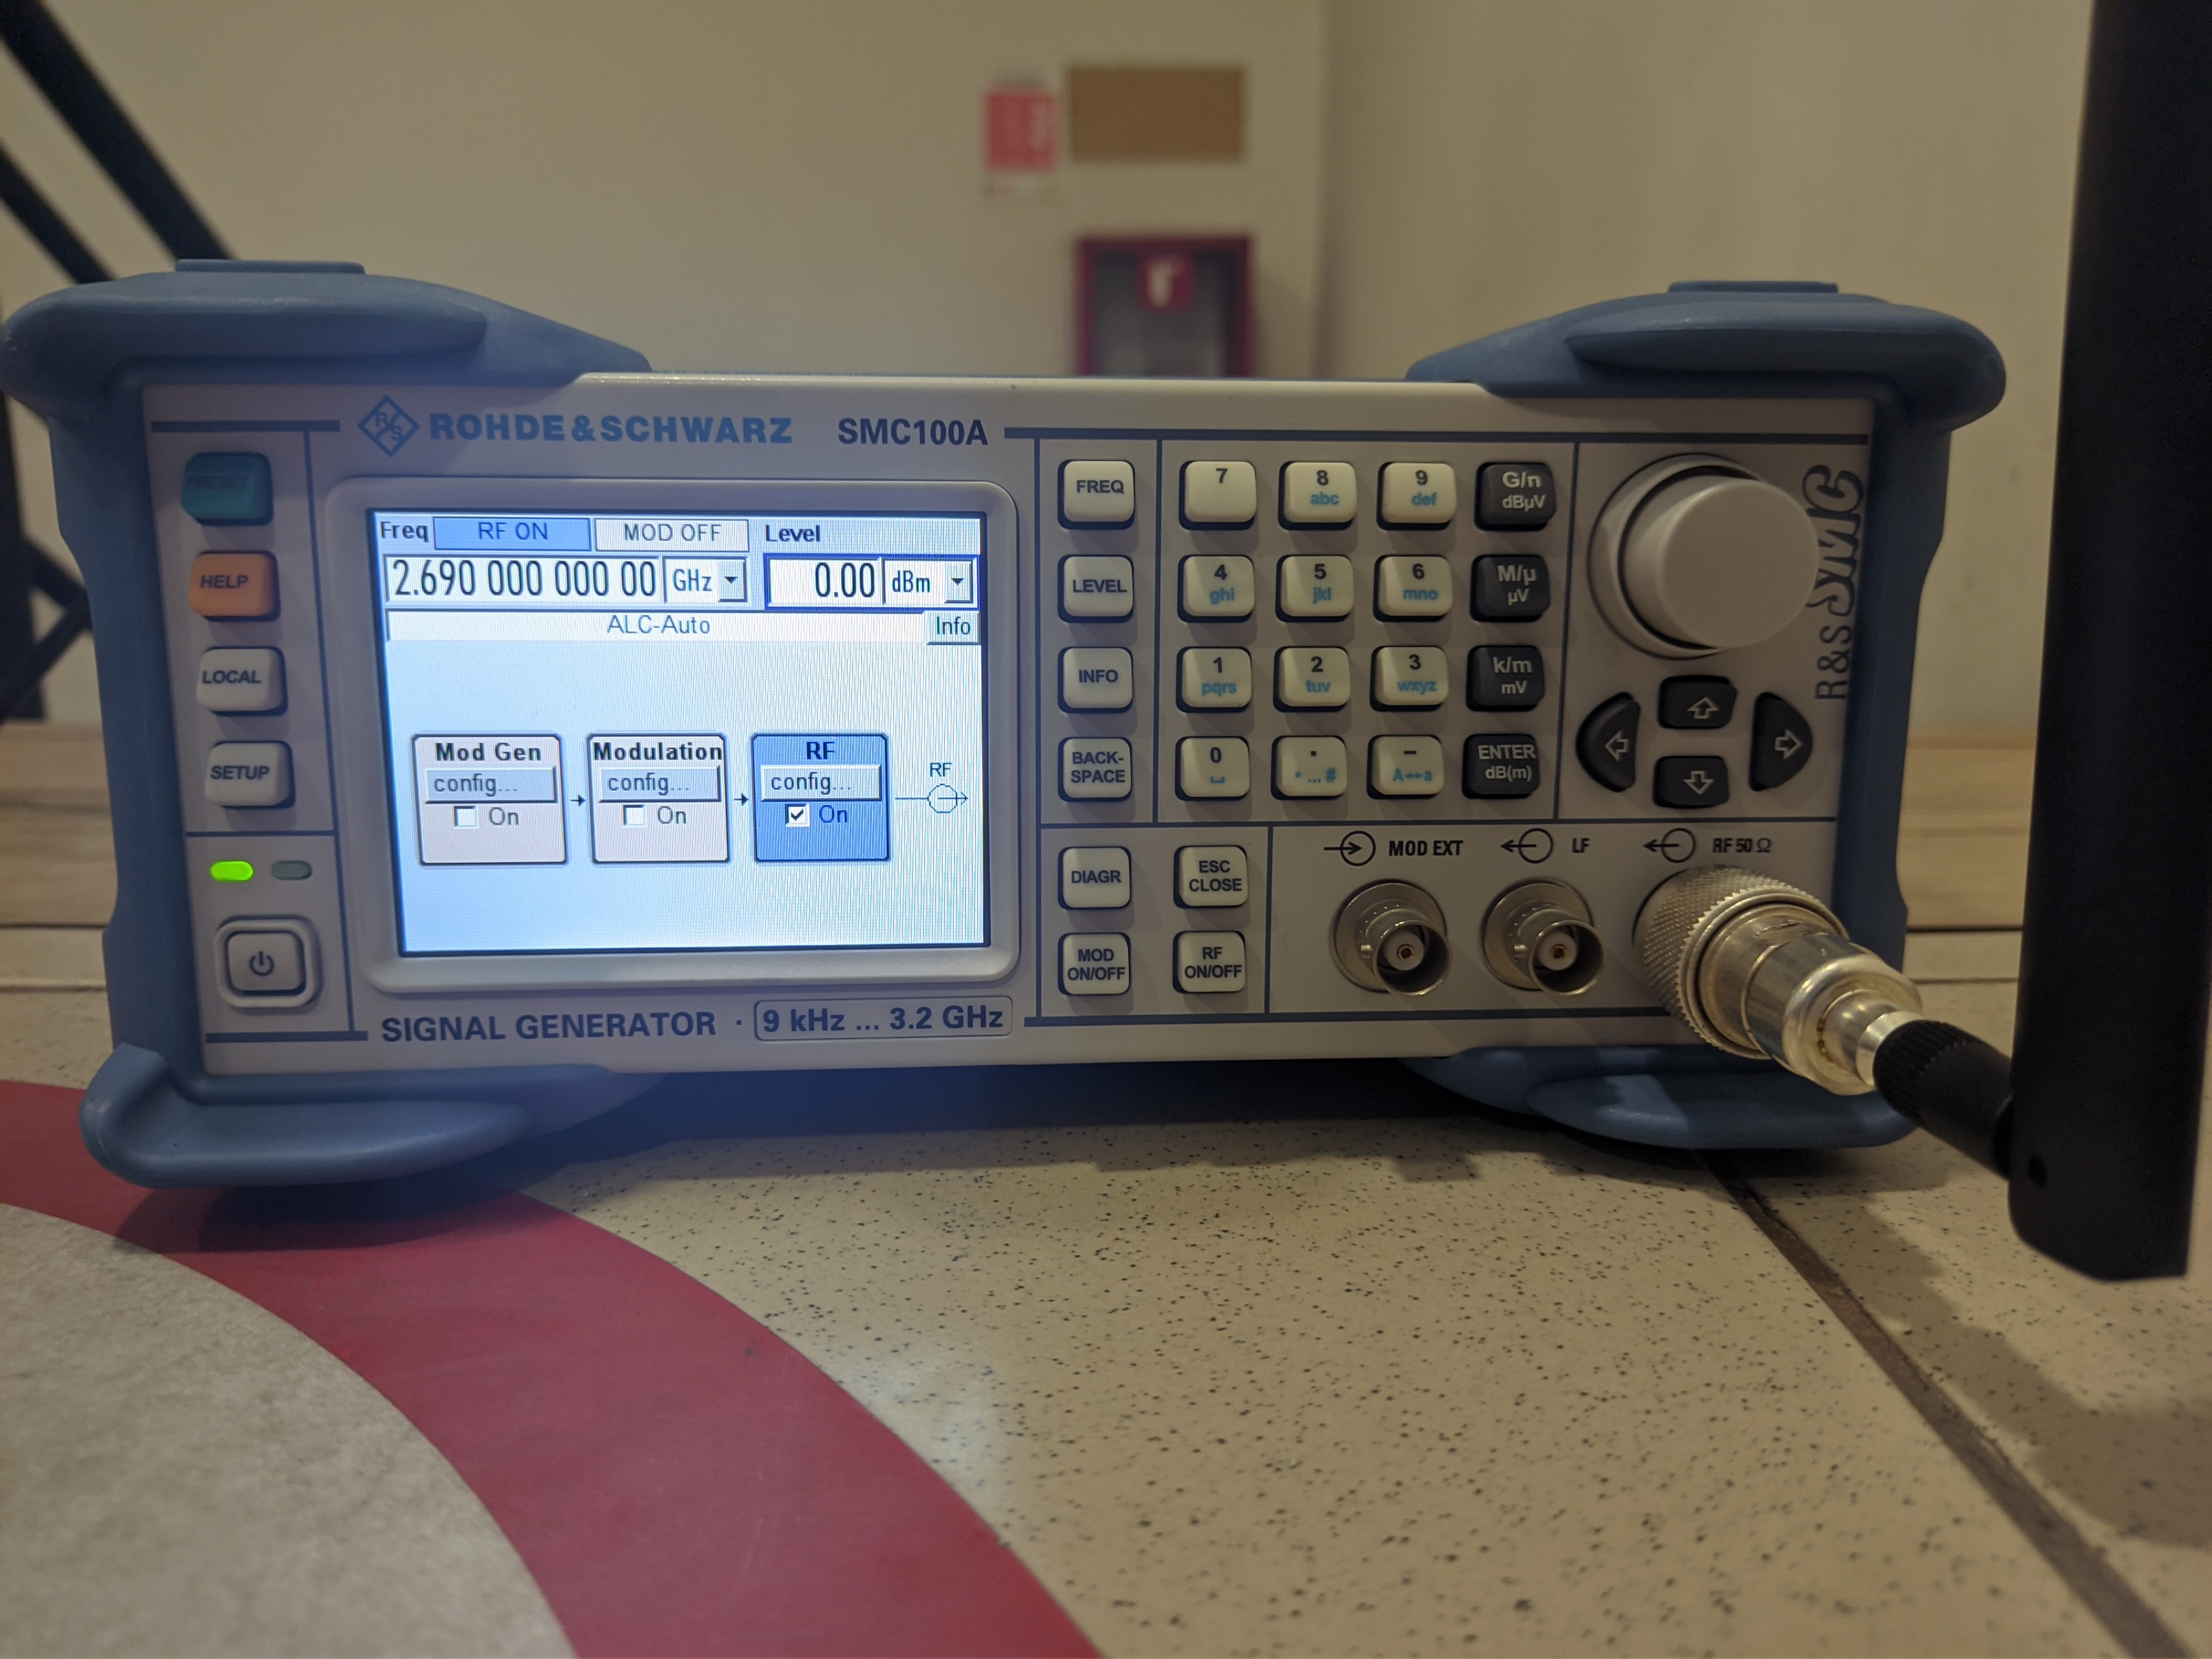
\includegraphics[width=\linewidth]{Imagenes/data/Transmisor.jpg}
        \caption{Transmisor}
        \label{transmisor}
  \end{figure}

  \begin{figure}[H]
        \centering
        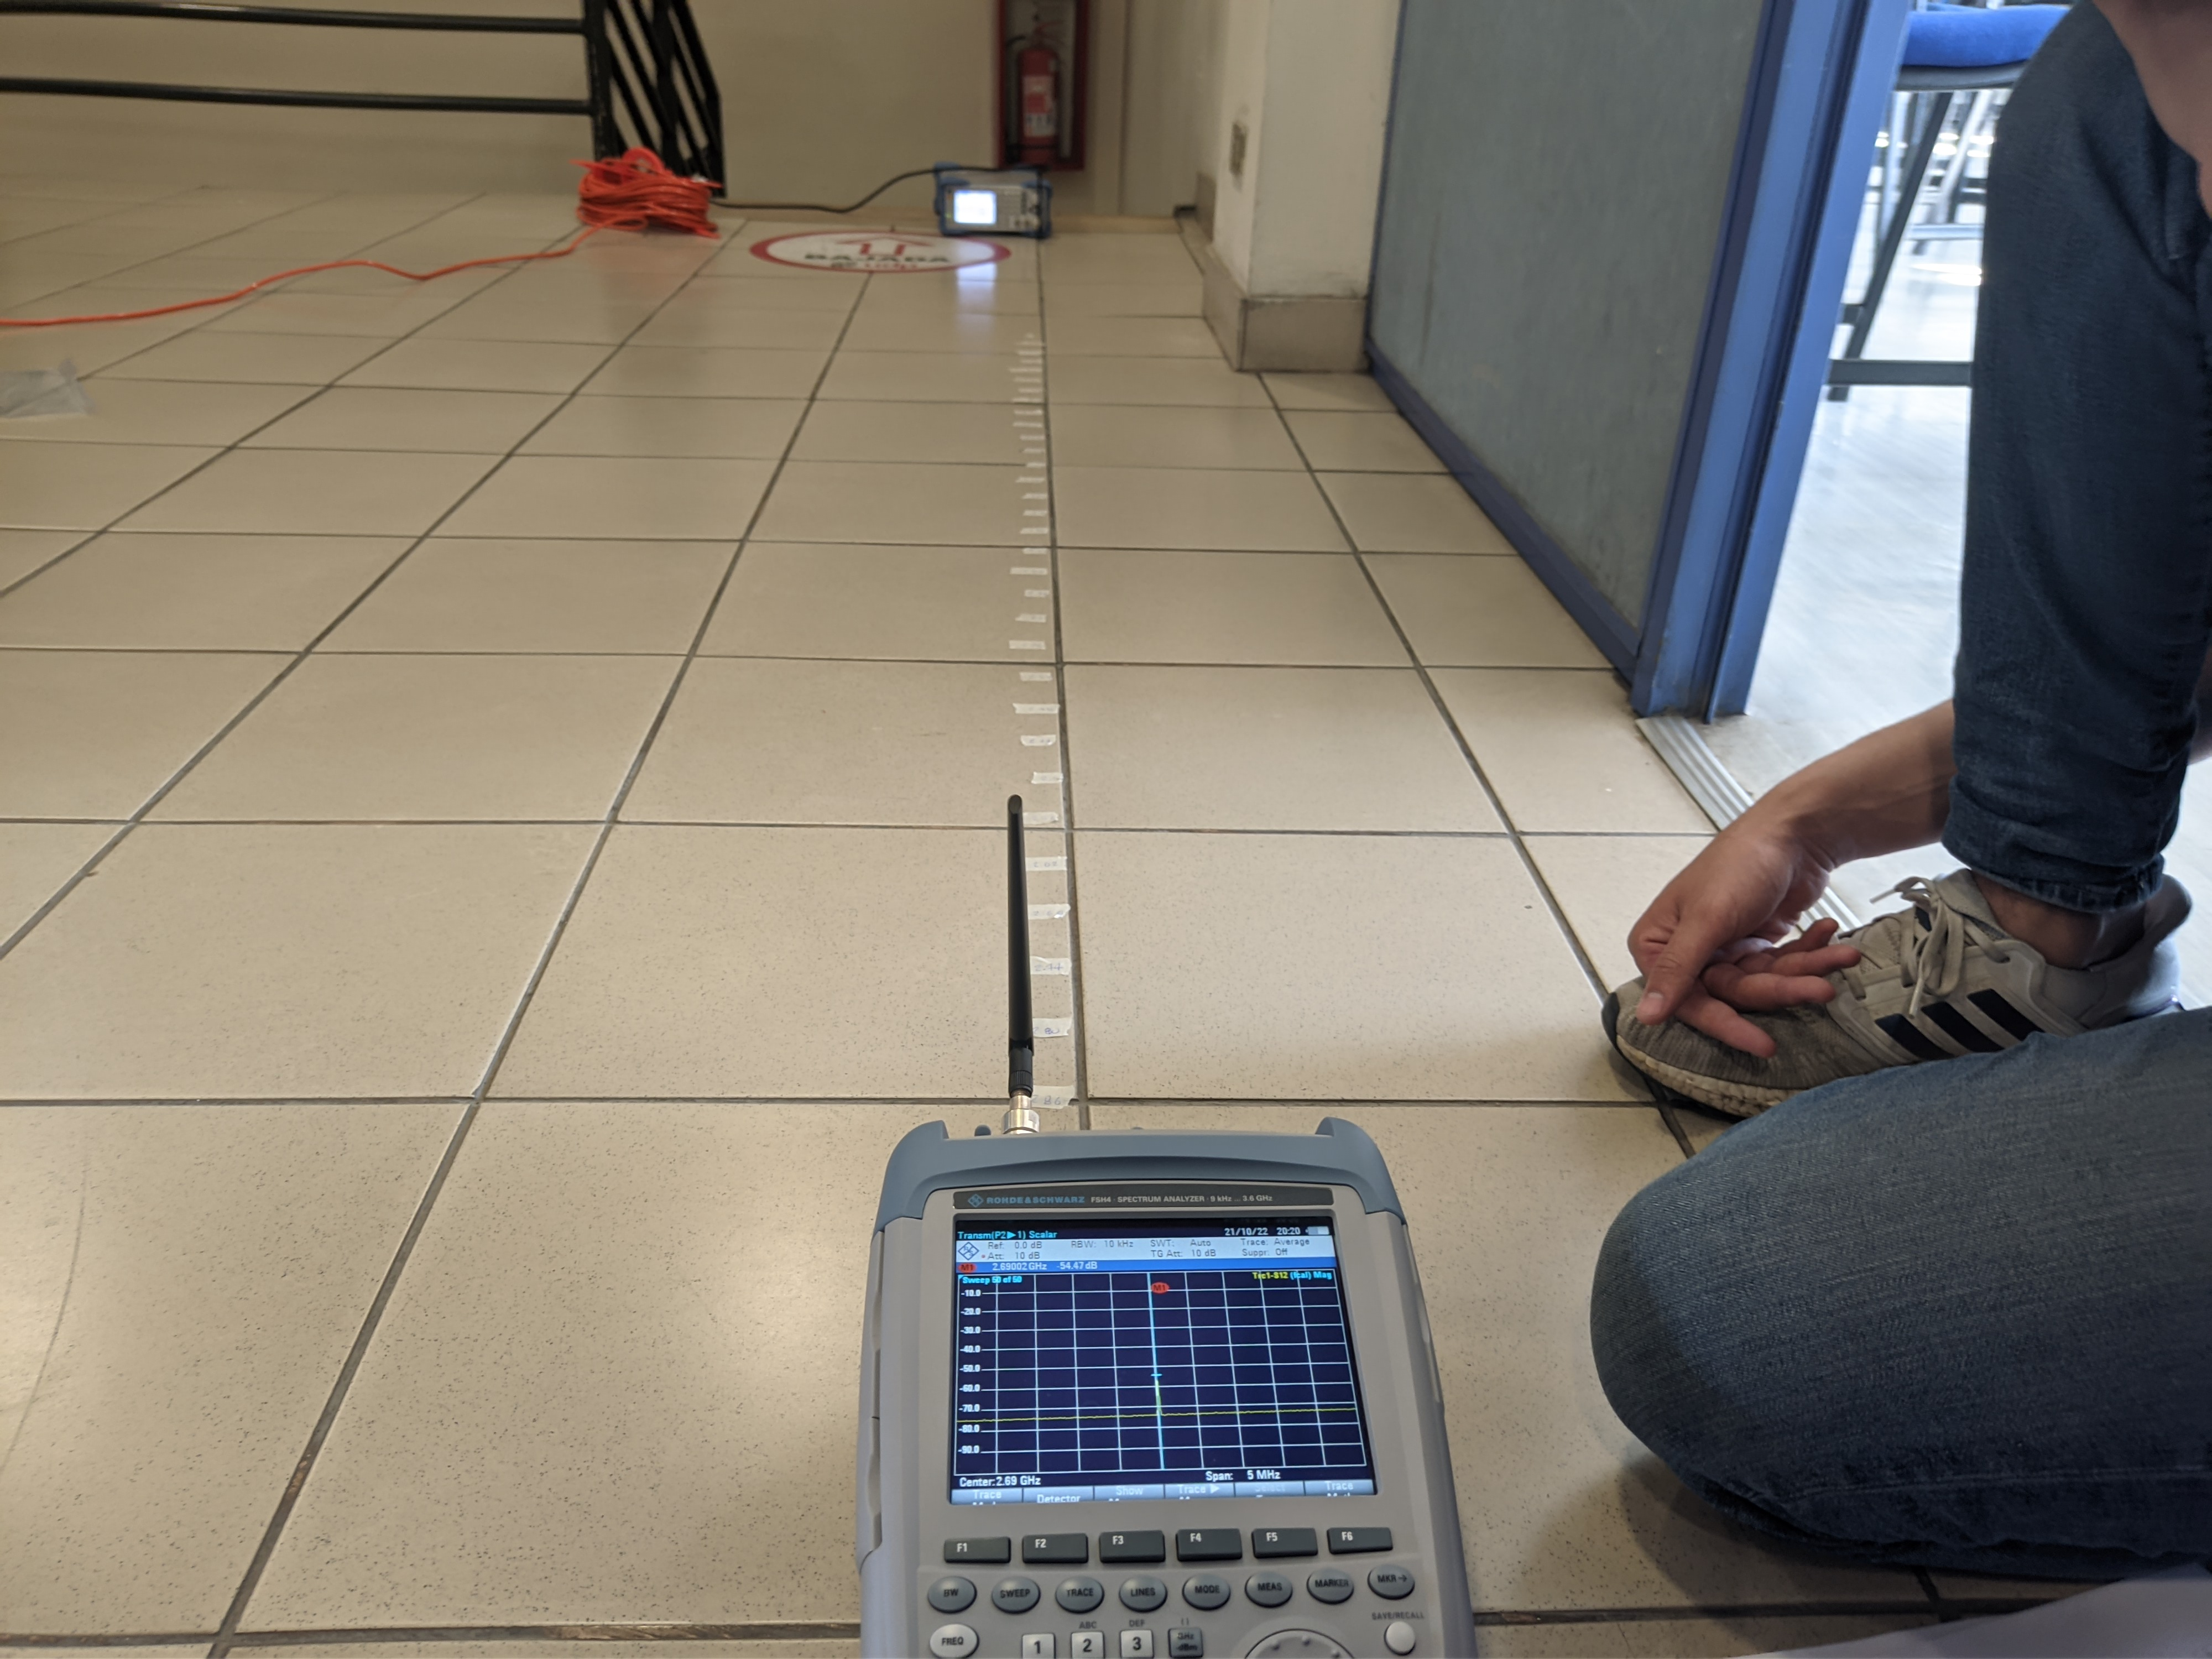
\includegraphics[width=\linewidth]{Imagenes/data/Fin_3metros.jpg}
        \caption{Perspectiva de medida hasta los 3 metros}
        \label{3m}
  \end{figure}

  \begin{figure}[H]
        \centering
        \includegraphics[scale=0.05, angle=-90]{Imagenes/data/Medida_lejana.jpg}
        \caption{Perspectiva de la medida más lejana posible medida(18 metros)}
        \label{18m}
  \end{figure}

\subsection{Gráfico de los resultados}

  \begin{figure}[H]
        \centering
        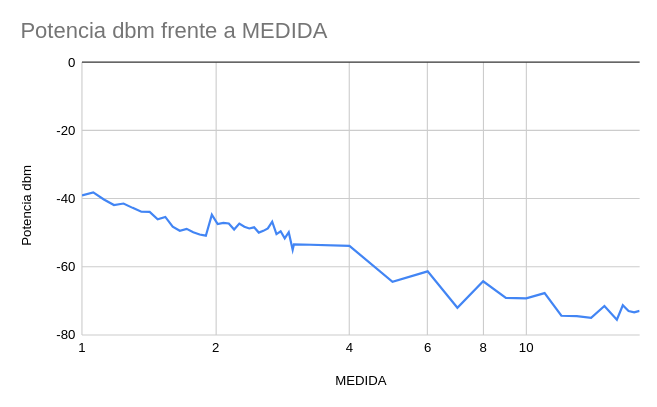
\includegraphics[width=\linewidth]{Imagenes/grafico.png}
        \caption{Distancia de medición vs Potencia dBm}
        \label{fig:grafico}
  \end{figure}
  \begin{figure}[H]
        \centering
        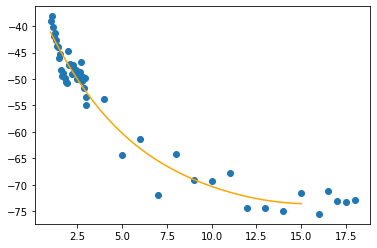
\includegraphics[width=\linewidth]{Imagenes/grafico con n.png}
        \caption{Con el n}
        \label{fig:grafico}
  \end{figure}
  
En el siguiente apartado, se adjunta el link donde se puede visualizar las distancias y potencias utilizadas para realizar el gráfico anterior.

\href{https://docs.google.com/spreadsheets/d/1fRkynR8ZBY9CO_3KUc9rnQAkz-86-G7ja93jMy49Xnk/edit?usp=sharing}{Click aquí}


La casilla b60 corresponde a la pendiente de la recta que mejor se ajusta a los datos, esta fue calculada mediante el método de mínimos cuadrados, y la casilla b61 corresponde al exponente de perdida. 